\documentclass[a4paper,14pt]{article}
\usepackage[export]{adjustbox}
\usepackage[colorlinks, linkcolor=blue]{hyperref}
\usepackage{indentfirst}

\usepackage[scaled]{DejaVuSansMono}
\usepackage[T1, T2A]{fontenc}



%\usepackage{helvet}
%\renewcommand{\familydefault}{\sfdefault}
\usepackage[utf8]{inputenc}
\usepackage[russian]{babel}

\usepackage{amsmath}
\usepackage{amssymb}
\usepackage{graphicx}
\usepackage{float}
\usepackage{sectsty}
\usepackage{fancyhdr}
\usepackage{titling}
\usepackage{datetime}
\usepackage{amsthm}
\usepackage[headheight=15pt]{geometry}
\usepackage{pstricks}
\usepackage{color}
\usepackage[linesnumbered, noline, noend]{algorithm2e}
\usepackage{caption}
\usepackage{subcaption}
\usepackage{verbatim}
\usepackage{amsfonts}
\usepackage{epstopdf}
\usepackage{mathtools}
\usepackage{wrapfig}
\usepackage{listings}
\usepackage{csvsimple}

\setlength{\droptitle}{-5em}

%opening
\title{Индивидуальное задание 2\\
	``Дискретизация сигнала и его спектральный анализ''\\
	Вариант 7}
\author{Илья Мурадьян, группа 4.1}

\sectionfont{\normalfont\centering\textbf}
\geometry{left=2cm}% левое поле
\geometry{right=1.5cm}% правое поле
\geometry{top=1cm}% верхнее поле
\geometry{bottom=2cm}% нижнее поле

\newcommand{\code}[1]{\begin{normalsize}\texttt{#1}\end{normalsize}}

\newcommand{\csvfreqtable}[3]{
	\begin{table}[H]
		\centering
		\csvreader[
			tabular=|c|c|c|c|,
			table head=\hline \textbf{№} & \textbf{Круговая частота} & \textbf{Частота, Гц} & \textbf{Амплитуда}\\\hline,
			late after line=\\\hline
		]{#1}{w=\csvw, nu=\csvnu, ampl=\csvampl}{\thecsvrow & \csvw & \csvnu & \csvampl}
		\caption{#2}
		\label{#3}
	\end{table}
}

\graphicspath{ {../} }
\floatstyle{boxed} 
\restylefloat{figure}

\lstset{basicstyle=\normalsize\ttfamily,breaklines=true}
\lstset{frame=single}
\lstdefinestyle{py}{
	language=Python, 
	captionpos=b,
	inputencoding=utf8,
	extendedchars=true
}

\theoremstyle{definition}
\newtheorem{defn}{Определение}

\begin{document}
	\Large
	
	\maketitle
	
	Мой вариант предполагал работу с сигналом $x_0, x_1, ..., x_{N - 1}, N = 512$ с частотой дискретизации $h \approx 0.018104$ из файла \code{Sa7.tx}. Ввиду того, что файл содержит 513 строк, я его здесь не привожу.
	\begin{figure}[H]%{l}{0.6\textwidth}
		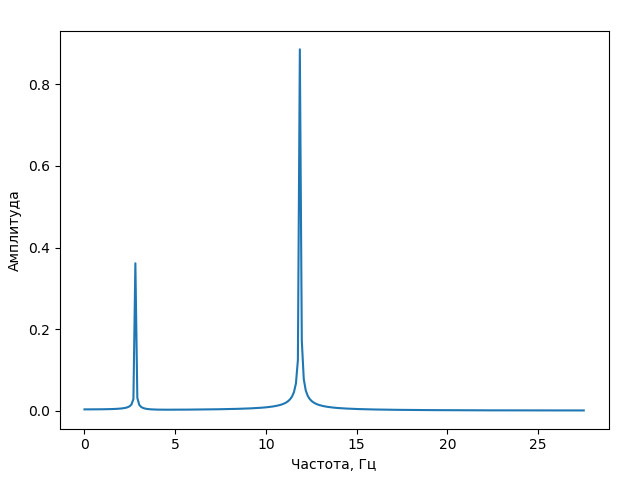
\includegraphics[width=0.8\linewidth, center]{Figure1} 
		\caption{БПФ исходного сигнала}
		\label{fig:f1}
	\end{figure}
	
	Было проведено преобразование Фурье $X_0, X_1, ..., X_{N - 1}$ входного сигнала, график функции $A_i = \frac{2 |X_i|}{N}, i = 0, 1, ..., \frac{N}{2} - 1$ приведён на рисунке \ref{fig:f1}. Нормировка вещественного сигнала понадобилась для получения реальных амплитуд. Частоты в герцах вычислялись через индексы следующим образом:
	\begin{equation}
		\nu_i = \frac{i}{N h}
	\end{equation}
	
	Для выделения гармоник была написана функция \code{extract\_harmonics} (см. листинг \ref{lst:exh}). Она выделяет амплитуды выше некоторого предела, устанавливаемого вручную (я всюду брал $threshold=0,2$), а затем в выделенных кусках находит максимумы и соответствующие им индексы.
	\begin{lstlisting}[style=py, caption={Функция extract\_harmonics}, label={lst:exh}]
def extract_harmonics(frequencies, amplitudes, threshold = None):
	th = threshold if threshold is not None else CONFIG['threshold']
	labels, num_labels = ndimage.label(amplitudes > th)
	unique_labels = np.unique(labels)
	idx = np.array(ndimage.maximum_position(amplitudes, labels, unique_labels[1:])).reshape((num_labels, ))
	return frequencies[idx], amplitudes[idx]
	\end{lstlisting} 
	
	По найденным частотам в герцах круговые частоты восстанавливались по формуле:
	\begin{equation}
	\omega_i = 2 \pi \nu_i.
	\end{equation}
	
	Это преобразование и печать данных о выделенных гармониках осуществляет функция \code{print\_components}, приведённая в листинге \ref{lst:pcomp}.
	\begin{lstlisting}[style=py, caption={Функция print\_components}, label={lst:pcomp}]
def print_components(title, frequencies, amplitudes):
	break_out = '='*60
	c_f = 2 * np.pi * frequencies
	print('\n{}:'.format(title))
	print(break_out)
	print('Circular freq\t\t\tFreq\t\t\t\t\tA')
	for i in range(frequencies.shape[0]):
		print('{}\t\t{}\t\t{}'.format(c_f[i], frequencies[i], amplitudes[i]))
		print(break_out)
		print('')
	\end{lstlisting} 
	
	В листинге \ref{lst:iofun} приведены ещё две вспомогательные функции, осуществляющие чтение из файла, сохранение графиков в файл и их вывод на экран.
	\lstinputlisting[style=py, caption={Функции ввода-вывода}, label={lst:iofun}, linerange={8-27}]{../lab2.py}
	
	Наконец, в листинге \ref{lst:clrmain} все указанные функции были использованы для выделения гармоник из исходного сигнала.
	\begin{lstlisting}[style=py, caption={Обработка исходного сигнала}, label={lst:clrmain}]
h, data = get_data()
n = data.shape[0]
n_2 = n // 2
t_all = n * h

freq_line = np.arange(n) / t_all
freq_line_2 = freq_line[:n_2]
data_t = np.fft.fft(data, n)
data_t_amplitudes = (np.abs(data_t) / n * 2)[:n_2]

show_save(freq_line_2, data_t_amplitudes, 'Figure1', 'Frequency, Hz', 'Amplitude')
harmonics_1 = extract_harmonics(freq_line_2, data_t_amplitudes)
print_components('Clear signal components', *harmonics_1)
	\end{lstlisting} 
	
	В таблице \ref{tab:clt} приведены амплитуды и частоты выделенных гармоник.
		
	\csvfreqtable{../clear.csv}{Чистый сигнал}{tab:clt}
	
	\begin{defn}
		Шумом амплитуды $A$ будем называть сигнал $x$, для которого $x_i = A \cdot rand(-1, 1)$. $rand(a, b)$ здесь означает случайную величину, равномерно распределенную на отрезке $[a, b]$.
	\end{defn}
	
	Поскольку шум носит случайный характер, указать на точную границу амплитуды, при которой из сигнала ещё можно выделить исходные гармонические составляющие, сложно. Но указать примерные границы можно. Получилось, что при амплитуде $A_1=1,5$ исходные гармоники ещё выделяются (см. рисунок \ref{fig:f2}, таблицу \ref{tab:oksig}), а при амплитуде $A_2=2$ -- уже нет (см. рисунок \ref{fig:f3}, таблицу \ref{tab:noksig}).
	
	\begin{figure}[H]%{l}{0.6\textwidth}
		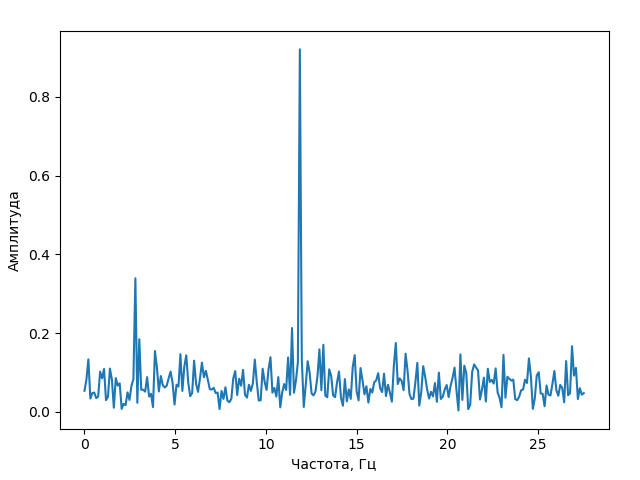
\includegraphics[width=0.6\linewidth, center]{Figure2} 
		\caption{Несильно зашумленный сигнал}
		\label{fig:f2}
	\end{figure}
	
	\csvfreqtable{../csvFigure2.csv}{Гармоники несильно зашумленного сигнала}{tab:oksig}
	
	\begin{figure}[H]%{l}{0.6\textwidth}
		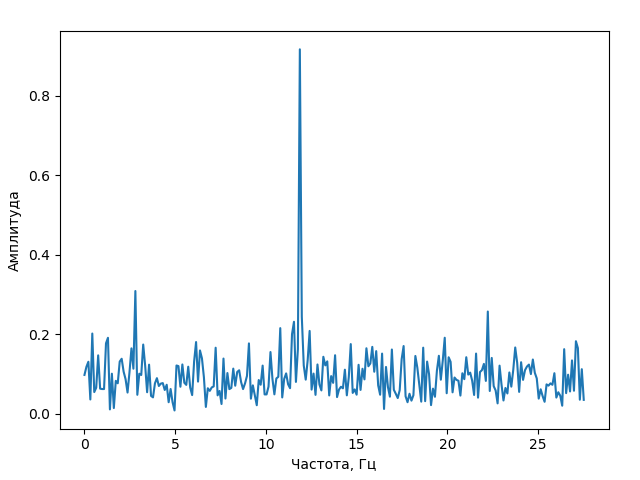
\includegraphics[width=0.6\linewidth, center]{Figure3} 
		\caption{Сильно зашумленный сигнал}
		\label{fig:f3}
	\end{figure}
	
	\csvfreqtable{../csvFigure3.csv}{Гармоники, выделенные программой в плохом сигнале}{tab:noksig}
	
	В листинге \ref{lst:noise} приведена работа с зашумленными сигналами: генерация шума, сложение сигналов, вычисление их БПФ и выделение гармоник.
	
	\begin{lstlisting}[style=py, caption={Работа с зашумленным сигналом}, label={lst:noise}]
noise_configs = [
	(1.5, 'Figure2', 'OK noise'),
	(2, 'Figure3', 'Not-OK noise'),
]

for noise_a, figure_title, log_title in noise_configs:
	noise = np.random.rand(n) * (noise_a * 2) - noise_a
	
	noised_signal = data + noise
	noised_t = np.fft.fft(noised_signal, n)
	noised_t_amplitudes = (np.abs(noised_t) / n * 2)[:n_2]
	
	show_save(freq_line_2, noised_t_amplitudes, figure_title, 'Frequency, Hz', 'Amplitude')
	harmonics_2 = extract_harmonics(freq_line_2, noised_t_amplitudes)
	print_components(log_title, *harmonics_2)
	\end{lstlisting}
	
	Прибавим теперь к нашему сигналу следующий сигнал:
	\begin{equation}
		\label{eq:newaddsig}
		\widehat{x}(t) = A\cos(\Omega_1 t) + 2 A\cos(\Omega_2 t)
	\end{equation}
	Амплитуду $A$ выберем равной $0,4$, чтобы амплитуды составляющих сигнал $\widehat{x}$ гармоник оказались между найденными нами амплитудами гармоник исходного сигнала (которые составляют примерно $0,36$ и $0,89$). Шаг дискретизации оставим таким же.
	
	Частота Найквиста для используемого нами шага дискретизации составляет:
	\begin{equation}\label{eq:nyqf}
		\nu_N = \frac{1}{2 h} \approx 27,61781.
	\end{equation}
	
	Круговая частота Найквиста составляет, соответствено:
	\begin{equation}\label{eq:nyqw}
		\omega_N = \frac{\pi}{h} \approx 173,5278.
	\end{equation}
	
	Необходимо выбрать частоты сигнала $\widehat{x}$ так, чтобы выполнялось $\Omega_1 < \Omega_2 < \omega_N$, или $\frac{\Omega_1}{2 \pi} <\frac{\Omega_2}{2 \pi} < \nu_N$. Поэтому возьмём $\nu_1 = \frac{\Omega_1}{2 \pi} = 25$, $\nu_2 = \frac{\Omega_2}{2 \pi} = 27$. Для полученного после сложения с исходным сигнала проведём преобразование Фурье. График можно видеть на рисунке \ref{fig:f4}. 
	
	\begin{figure}[H]
		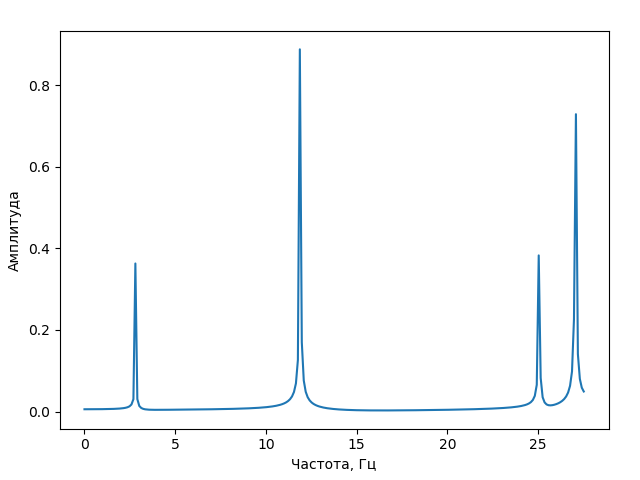
\includegraphics[width=0.8\linewidth, center]{Figure4} 
		\caption{Модифицированный сигнал}
		\label{fig:f4}
	\end{figure}
	
	В таблице \ref{tab:modaddsig} можно видеть, что программа распознала все 4 частотных пика.	
	\csvfreqtable{../csvFigure4.csv}{Гармоники модифицированного сигнала}{tab:modaddsig}
	
	Если $\Omega_2 > \omega_N$, возникает алиасинг. При дальнейшем увеличении $\Omega_2$ пики добавляемых гармоник меняются местами. В теории это должно происходить, когда $\Omega_2 > \omega_N + (\omega_N - \Omega_1) = 2 \omega_N - \Omega_1 \approx 189,976$. На практике приходится брать значения ещё больше, чтобы получилась хорошая картинка. Было взято значение $\Omega_2 = 33\cdot 2 \pi \approx 207,345$. Получились график \ref{fig:f5} и таблица \ref{tab:alisig}.
	
	\begin{figure}[H]
		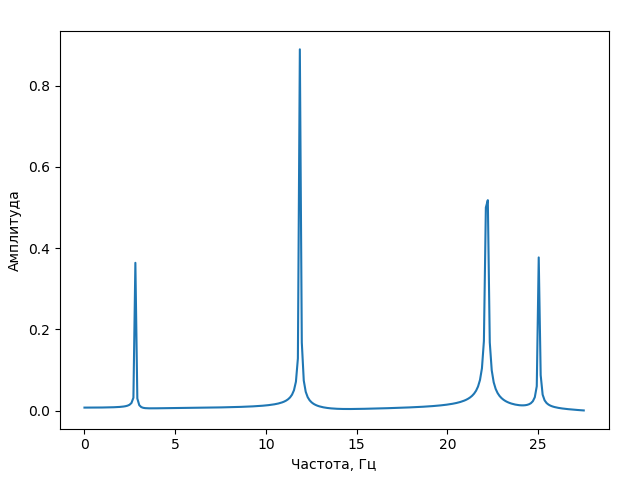
\includegraphics[width=\linewidth, center]{Figure5} 
		\caption{Алиасинг}
		\label{fig:f5}
	\end{figure}
	
	\csvfreqtable{../csvFigure5.csv}{Гармоники при алиасинге}{tab:alisig}
	
	Если уменьшить шаг дискретизации до $h' = \frac{h}{2}$ и взять $\Omega_1 = 20 \cdot 2 \pi, \Omega_2 = 25 \cdot 2 \pi$ (то есть взять такие круговые частоты, с которыми при шаге дискретизации $h$ алиасинга не возникало), то возникнет алиасинг. Соответствующие график и таблица приведены ниже.
	
	\begin{figure}[H]
		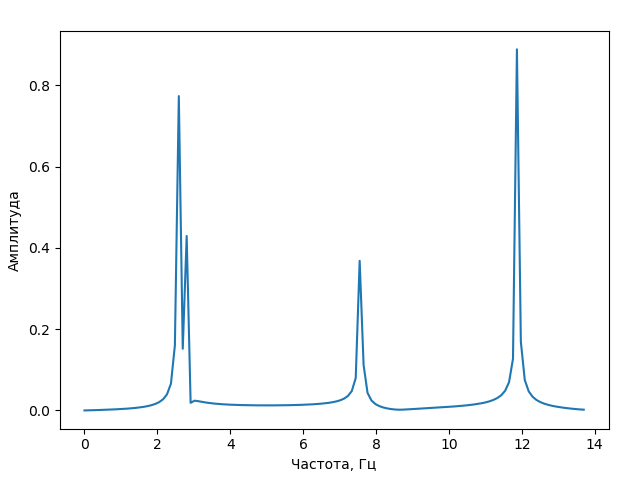
\includegraphics[width=\linewidth, center]{Figure6} 
		\caption{Алиасинг при маленьком шаге дискретизации}
		\label{fig:f6}
	\end{figure}
	
	\csvfreqtable{../reduced.csv}{Гармоники огрублённого сигнала, алиасинг}{tab:aliredsig}
	
	Остаток программы, который рисует три последние картинки/таблицы, приведён в листинге \ref{lst:reduced}.
	\begin{lstlisting}[style=py, caption={Работа с модифицированным сигналом}, label={lst:reduced}]
add_amplitude = CONFIG['add_amplitude']
add_configs = [
	(25, 27, 'Figure4', 'Modified signal (no aliasing)'),
	(25, 33, 'Figure5', 'Modified signal (aliasing + strange behavior)'),
]

for s1, s2, figure_title, log_title in add_configs:
	add_signal = modified_signal(time_line, s1, s2, add_amplitude)
	mod_sig = data + add_signal
	mod_t = np.fft.fft(mod_sig, n)
	mod_t_a = (np.abs(mod_t) / n * 2)[:n_2]
	
	show_save(freq_line_2, mod_t_a, figure_title, 'Frequency, Hz', 'Amplitude')
	harmonics_4 = extract_harmonics(freq_line_2, mod_t_a)
	print_components('csv'+figure_title, log_title, *harmonics_4)

add_signal = modified_signal(time_line, 20, 25)
mod_sig2 = add_signal[::2] + data[::2]
freq_line_4 = (np.arange(n//2) / (n * h))[:n//4]
mod_t2 = np.fft.fft(mod_sig2)
mod_t_a2 = (np.abs(mod_t2) / (n//2) * 2)[:n_2//2]

show_save(freq_line_4, mod_t_a2, 'Figure6', 'Frequency, Hz', 'Amplitude')
harmonics_6 = extract_harmonics(freq_line_4, mod_t_a2)
print_components('reduced','Modified signal components (only even samples)', *harmonics_6)
	\end{lstlisting}
	
	Работа была выполнена мною лично, без чьей-либо помощи, без использования нелицензионных программ.
	
\end{document}
